\documentclass[10pt,a4paper]{article}
\usepackage[utf8]{inputenc}
\usepackage[french]{babel}
\usepackage[T1]{fontenc}
\usepackage{amsmath}
\usepackage{amsfonts}
\usepackage{amssymb}
\usepackage{graphicx}
\usepackage[left=2cm,right=2cm,top=2cm,bottom=2cm]{geometry}
\usepackage{hyperref}
\usepackage{listings}

\title{L.A.R.A Documentation}
\author{Rédigé par : Louis Grenioux, Anna-Rose Lescure, Riad El Otmani}

\newcommand\tab[1][0.5cm]{\hspace*{#1}}

\begin{document}

\maketitle
\tableofcontents

\section{Facebook Parser}
\subsection{Objectifs et outils}
Nous avons décidé de travailler tout au long de ce projet en ayant comme objectif d'entraîner notre programme sur nos données personnelles, extraites notamment de nos conversations Facebook. Ainsi le parser qui a été développé est l'un des module critique qui forme la version actuelle de L.A.R.A.

Son rôle est d'ordonner et organiser le dump de données que nous pouvons télécharger sur facebook de manière à en faire un dataset d'entraînement et de validation valide pour les prochains modules de la chaîne.
\subsection{Traitement des données}
Le parser opère sur le dump FaceBook un ensemble d'opérations dont il est possible de voir le résultat dans cette partie.
\subsubsection{Données initiales}
Données extraites du fichier \texttt{dumpFacebook.json}.
\begin{verbatim}
...
{
    "sender_name": "Riad El Otmani",
    "timestamp_ms": 1579199706153,
    "content": "J'ai des trains \u00c3\u00a0 15",
    "type": "Generic"
},
{
    "sender_name": "Louis Popi",
    "timestamp_ms": 1579199562206,
    "content": "C'est une bonne marge de s\u00c3\u00a9curit\u00c3\u00a9",
    "type": "Generic"
}
...
\end{verbatim}

\subsubsection{Données finales}
Données produites par le parser après traitement.
\begin{verbatim}
...
{
   "sender_name":"Louis Popi",
   "content":"c'est une bonne marge de securite",
   "conversationId":4,
   "subConversationId":27
},
{
   "sender_name":"Riad El Otmani",
   "content":"j'ai des trains a  15",
   "conversationId":3,
   "subConversationId":27
}
...
\end{verbatim}
\subsection{Programme}
\subsubsection{Constructeur de la classe \texttt{Parser}}
Le parser facebok est construit autour d'une classe \texttt{Parser}. Son constructeur initialise les variables de la classe avec les valeurs qui lui sont transmises et s'occupe de charger en mémoire le contenu du dump téléchargé sur Facebook.  Voici son constructeur :
\begin{center}
	\texttt{\_\_init\_\_(self, fileName, nbMessages, delayBetween2Conv, answerer, withTimestamp=True, debug=False)}
\end{center}


\begin{itemize}
  \item \texttt{fileName} : donne le chemin d'accès au fichier de données à parser qui sera utilisé par la suite.
  \item \texttt{nbMessage} : correspond aux nombres de messages qui vont être traités par le parser.
  \item \texttt{delayBetween2Conv} : indique une durée arbitraire qui permet de délimiter les conversations.
  \item \texttt{answerer} : indique la personne qui aux questions
  \item \texttt{withTimeStamp} : option qui permet l'utilisation ou non des timestamps.
  \item \texttt{debug} : mode debuggage.
\end{itemize}

\subsubsection{La méthode \texttt{start}}
La méthode \texttt{start} est l'une des methodes les plus importante de la classe, elle ne prend aucun argument. Elle initialise deux listes \texttt{self.conversation['speakers']} et \texttt{self.conversation['messages']} qui contiendront respectivement la liste des participants à la conversation et ainsi que son contenu.

Dans un premier temps, on remplit la liste \texttt{conversation.['speakers']} simplement en se basant sur le champ \texttt{conversation['participants']} du dump JSON. Vient ensuite le problème de la gestion des messages. Dans un premier temps, nous devons vérifier l'utilisabilité du dump.

Pour cela on itère sur chaque élément du dump et on vérifie que l'élément en question est bien un message en utilisant la methode \texttt{self.getMsg()}. Dans le cas où c'est bien un message on peut l'ajouter dans la liste \texttt{self.conversation['message']}, dans le cas contraire on émet un message d'erreur.

Au vu de la grande variété possible des différents messages (text, emoji, réaction, image, vidéo, ...), nous devons passer par une phase de nettoyage en amont afin de réduire nos données à quelque chose d'utilisable par les autres modules et notamment pour le réseau de neuronnes.

On décide ainsi de trier les messages par leur timestamps afin de les ordonner temporellement sous forme de conversations. Pour réaliser cette séparation, on se base sur l'écart de temps entre les différents messages car on part du principe que le RNN sera plus performant en travaillant par conversations puisque les messages seront liés entre eux par le contexte de la conversation.

\begin{center}
    \texttt{if abs(int(self.dataRaw['messages'][k]['timestamp\_ms']) - timestamp) > self.delayBetween2Conv}
\end{center}

Pendant la création de la conversation, repérée par son \texttt{id}, on vérifie certaines conditions pour assurer la validité de la conversation. 

Ainsi, une nouvelle conversation doit obligatoirement commencer par une question et la conversation précédente doit terminer par une réponse. On fera aussi attention à éviter les conversations de type monologue où il n'y a pas d'échange entre les deux participants. Quand une de ces conditions n'est pas vérifiée, on supprime simplement la conversation en question.

Voici une représentation simplifiée de l'attribution des \texttt{ids} par le parser :

\begin{verbatim}
(ID = 0 | SID = 0) Riad : Salut
(ID = 0 | SID = 1) Louis : Salut
(ID = 0 | SID = 2) Riad : ça va ?
(ID = 0 | SID = 3) Louis : oui et toi ?
(ID = 0 | SID = 3) Louis : tu fais quoi ?
[20 minutes plus tard]
(ID = 1 | SID = 0) Riad : je travaille sur le parser et toi ?
(ID = 1 | SID = 1) Louis : je m'occupe du nlp
\end{verbatim}

\subsubsection{La méthode \texttt{isAnswerer}}
Voici les paramètres : \texttt{isAnswerer(self, name)}. Il s'agit d'une methode simple qui renvoie un boolean résultant de cette opération : \texttt{name == self.answerer}.

\subsubsection{La méthode \texttt{removeFullConv}}
Voici les paramètres : \texttt{removeFullConv(self, conv\_id)}. Cette methode permet de supprimer une conversation entière grâce à son \texttt{id}.

\subsubsection{La méthode \texttt{removeSubConv}}
Voici les paramètres : \texttt{removeSubConv(self, conv\_id, subconv\_id)}. Cette methode permet de supprimer un message d'une conversation grâce à son \texttt{id}.

\subsubsection{La méthode \texttt{getMsg}}
Voici les paramètres : \texttt{getMsg(self, k, conversationId, subConversationId)}. Cette methode se charge de renvoyer un message structuré de type dictionnaire selon python. 

Voici un extrait du code :
\begin{lstlisting}[language=Python]
if self.withTimestamp:
	msg = {
	'sender\_name': self.dataRaw['messages'][k]['sender\_name'],
	'content': self.cleanMessage(self.dataRaw['messages'][k]['content']),
	'timestamp': self.dataRaw['messages'][k]['timestamp\_ms'],
	'conversationId': conversationId,
	'subConversationId': subConversationId
}
\end{lstlisting}

Si le champ \texttt{self.withTimestamp} vaut \texttt{False}, il suffit de retirer cette ligne. Dans le cas où le le message reçu n'est pas interpretable (message video, audio, réaction, ...) alors la fonction \texttt{self.cleanMsg} renvoie une erreur qui nous fait sortir d'un \texttt{try} nous permettant ainsi de pouvoir catch l'erreur dans le \texttt{except} et de supprimer ce message.

On renvoie finalement soit \texttt{msg} si tout s'est bien déroulé, soit l'\texttt{id} du message qui a causé l'erreur.

\subsubsection{La méthode \texttt{cleanMsg}}
Voici les paramètres : \texttt{cleanMessage(self, message)}. Cette methode renvoie le message sous forme de chaîne de caractères après avoir subit quelques transformations. Le but étant de transformer les caractères encodés par Facebook et de supprimer les majuscules du text.

\subsubsection{La méthode \texttt{extract\_time}}
Voici les paramètres : \texttt{extract\_time(self, msg)}. Cette méthode renvoie le timestamp associ au message. Dans le cas où celui-ci n'est pas défini, on renvoie la valeur \texttt{0}.

\subsubsection{La méthode \texttt{getNbConversation}}
Voici les paramètres : \texttt{getNbConversation(self)}. Cette méthode renvoie le nombre de messages enregistrés dans la lists \texttt{self.conversations['messages']}.

\subsubsection{La méthode \texttt{finalDump}}
Voici les paramètres : \texttt{finalDump(self, filename)}. Cette méthode créée le fichier \texttt{.json} final qui sera utilisé par les autres modules.

\subsection{Utilisation}
\subsubsection{Le parser}
Le parser a été conçu pour être utilisable le plus simplement possible. Pour cela une utilisation par ligne de commande a été implantée grâce à la librairie \texttt{argparse}.

Il suffit d'ouvrir un terminal et de lancer la commande :

\begin{center}
    \texttt{\$ python3 parserFB.py inputFile outputFile answerer}
\end{center}

Cette commande peut-être enrichie en donnant des arguments supplémentaires optionnels :

\begin{center}
    \texttt{\$ python3 parserFB.py inputFile outputFile answerer --nbMessages [int] --debug [True/False] --withTimestamp [True/False] --delayBetween2Conv [int]}
\end{center}

Voici ce que renvoie la commande \texttt{\$ python3 parserFB -h}.

\begin{verbatim}
positional arguments:
  inputFile             Path to input file containing facebook data
  outputFile            Path to output file
  answerer              Who will answer your questions

optional arguments:
  -h, --help            show this help message and exit
  --nbMessages [integer]
                        Default: 100
  --debug [True/False]  Default: False
  --withTimestamp [True/False]
                        Default: False
  --delayBetween2Conv [time_in_seconds]
                        Default: 20min

\end{verbatim}
\subsubsection{Les scripts BASH}
Le script \texttt{script\_parsing.sh} permet d'utiliser le parser sur toutes les conversations d'un dump Facebook. Son utilisation est la suivante :
\begin{center}
\texttt{./script\_parsing.sh fb\_folder out\_folder answerer fb\_parser}
\end{center}
où
\begin{itemize}
\item \texttt{fb\_folder} est le dossier de décompression du dossier Facebook ;
\item \texttt{out\_folder} est le dossier où les fichiers "parsés" seront stockés ;
\item \texttt{answerer} est le nom de la personne qui répond aux questions ;
\item \texttt{fb\_parser} est le chemin vers le script python.
\end{itemize}
L'intégralité des fichiers qui ont été traités peuvent maintenant être lu par le NLP avec \texttt{script\_java\_format} qui s'utilise comme suit :
\begin{center}
\texttt{./script\_java\_format.sh in\_folder out\_folder answerer java\_lib}
\end{center}
où
\begin{itemize}
\item \texttt{in\_folder} est le dossier contenant les sorties du parser (précédemment appelé \texttt{out\_folder}) ;

\item \texttt{out\_folder} est le dossier où seront stockés les résultat du NLP ; 
\item \texttt{answerer} est le nom de la personne qui répond aux questions ;
\item \texttt{java\_lib} est le chemin vers le \texttt{jar} du NLP (de lara).
\end{itemize}
\section{Natural Langage Processing - NLP}
\subsection{Objectifs et outils}
L'objectif du module NLP est double : il doit à la fois faire toute la partie de préparation des données qui seront ensuite mises à la disposition du RNN et il doit faire toute la partie de langage processing en entraînant des algorithmes de Word2Vec. Ce package (\texttt{org.lara.nlp}), dont le code source individuel peut être retrouvé \href{https://github.com/LaraProject/nlp}{ici}, est compilé avec le logiciel Maven et fait majoritairement appel à la bibliothèque open-source de référence en Deep-Learning : \href{https://deeplearning4j.konduit.ai/}{Deeplearning4J}.
\subsection{La classe \texttt{Context}}
La classe abstraite \texttt{Context} (\texttt{org.lara.nlp.context.Context}) permet de réaliser la préparation des données. Elle a été implémentée par deux classes filles : \texttt{Facebook}, qui exploite les données issues du parser et \texttt{Cornell}, qui exploite les données issues du \href{https://www.cs.cornell.edu/~cristian/Cornell_Movie-Dialogs_Corpus.html}{corpus de Cornell}. L'objectif est de fournir à partir de ces différentes sources deux listes de même taille : l'une contenant les questions et l'autre des réponses ; toutes deux parfaitement nettoyées (nous détaillerons ce nettoyage plus tard). \\
\tab La méthode \texttt{init()} permet d'initialiser l'objet en remplissant ces deux listes. Les deux listes peuvent ensuite être "tokenizées" (cf RNN) avec \texttt{tokenize()} ou nettoyées \texttt{cleaning()} (cf \texttt{Processer}). \\
\tab Les données peuvent être exportées et importées avec les méthodes \texttt{save(String path\_questions, String path\_answers)} et \texttt{restore(String path\_questions, String path\_answers)}. Il est aussi possible d'exporter ces deux listes dans un même fichier via \texttt{exportData(String path)} (cette méthode sera utilisée dans pour le RNN).
\subsubsection{La classe \texttt{Cornell}}
La classe \texttt{Cornell} implémente \texttt{Context} pour le \href{https://www.cs.cornell.edu/~cristian/Cornell_Movie-Dialogs_Corpus.html}{corpus de Cornell}. Son contructeur est
\begin{center}
 \texttt{Cornell(String lines\_filename, String conversations\_filename, int min\_length, int max\_length)}
\end{center}
où
\begin{itemize}
\item \texttt{min\_length} et \texttt{max\_length} sont des paramètres destinés à la classe \texttt{Processer} ;
\item \texttt{lines\_filename} est le chemin du fichier \texttt{movie\_lines.txt} ;
\item \texttt{conversations\_filenames} est le chemin du fichier \texttt{movie\_conversations.txt}.
\end{itemize}
\tab Lors de l'appel à \texttt{init()} les listes \texttt{questions} et \texttt{answers} vont être remplies par tous les dialogues possibles apparaissant dans le corpus.
\subsubsection{La classe \texttt{Facebook}}
La classe \texttt{Cornell} implémente \texttt{Context} à partir des données issues du parser grâce à la bibliothèque \texttt{org.json.simple}. Son constructeur est
\begin{center}
\texttt{Facebook(String json\_filename, String answerer, int min\_length, int max\_length)}
\end{center}
où
\begin{itemize}
\item \texttt{min\_length} et \texttt{max\_length} sont des paramètres destinés à la classe \texttt{Processer} ;
\item \texttt{json\_filename} est le chemin du fichier issu du parser ;
\item \texttt{answerer} est le nom de la personne qui répond aux questions.
\end{itemize}
\tab  Lors de l'appel à \texttt{init()} les listes \texttt{questions} et \texttt{answers} vont être remplies en parcourant le fichier JSON avec les différentes variables exportées par le parser.
\subsubsection{La classe \texttt{Simple}}
La classe \texttt{Simple} implémente \texttt{Context} à partir d'un format de donnée très simple (sui est d'ailleurs celui exporté par \texttt{exportData(String path)} évoquée précédemment) :
\begin{center}
\texttt{Question: \ldots} \\
\texttt{Answer: \ldots} \\
\texttt{Question: \ldots} \\
\texttt{Answer: \ldots} \\
\end{center}
Son constructeur est 
\begin{center}
\texttt{public Simple(String filename, int min\_length, int max\_length)}
\end{center}
où
\begin{itemize}
\item \texttt{min\_length} et \texttt{max\_length} sont des paramètres destinés à la classe \texttt{Processer} ;
\item \texttt{filename} est le fichier contenant les conversations.
\end{itemize}
\tab  Lors de l'appel à \texttt{init()} les listes \texttt{questions} et \texttt{answers} vont être remplies en parcourant le fichier de conversations.
\subsubsection{La classe \texttt{Processer}}
La classe \texttt{Processer} est liée à la classe \texttt{Context}. Elle met en œuvre les méthodes permettant de nettoyer les données :
\begin{itemize}
\item \texttt{clean\_text(String orig)} cette fonction centrale renvoie une chaîne de caractère où plusieurs changements ont été effectués :
\begin{itemize}
\item les lettres du texte deviennent des minuscules ;
\item les URLs sont supprimées ;
\item la langue anglaise est simplifiée ("you're" devient "you are" par exemple) ;
\item les balises HTML sont enlevées ;
\item les emojis sont remplacés par leur signification (via la bibliothèque `emoji4j` qui peut être retrouvée ici \href{https://github.com/kcthota/emoji4j}{ici}) ;
\item la ponctuation est traitée par des expressions régulières ;
\item les caractères de terminaison de ligne sont supprimés.
\end{itemize}
\item \texttt{cleanQuestionsAnswers()} applique la fonction précédente à toutes les questions et les réponses ;
\item \texttt{lengthFilter()} supprime les couples question/réponse où l'un ou l'autre a un nombre de mots inférieur à \texttt{min\_length} ou supérieur à \texttt{max\_length} ;
\item \texttt{tokenize\_sentence(String s)} applique la tokenisation en ajoutant les tokens \texttt{<START>} et \texttt{<END>} au début et à la fin de la phrase et en rajoutant le mot \texttt{<PAD>} pour que la phrase ait une longueur égale à \texttt{max\_length} ;
\item \texttt{tokenize()} applique \texttt{tokenize\_sentence} à chaque question et à chaque réponse ;
\item \texttt{process()} applique le filtre de longueur et le nettoyage à chaque question et à chaque réponse.
\end{itemize}
\subsubsection{Le parser LELU}
\href{https://www.kaggle.com/breandan/french-reddit-discussion}{LELU} est un dataset disponible sur \href{https://www.kaggle.com/breandan/french-reddit-discussion}{Kaggle} qui regroupe $556,621$ conversations issues de Reddit. Le script \texttt{parserLELU.py} qui peut être retrouvé dans le repository \href{https://github.com/LaraProject/parserLELU}{LaraProject/parserLELU} ouvre les données de LELU et produit (via \texttt{stdout}) un fichier avec le format de \texttt{Simple}. Ce dataset sera utilisé pour l'entraînement du Word2Vec.

\subsection{Les implémentations de d'algorithme de plongement lexical}
Le NLP est aussi responsable de la tâche de plongement lexical (word embedding). Il implémente plusieurs algorithmes de \texttt{Word2Vec} via des classes très similaires mais sans héritage commun explicite. Ces classes utilisent pleinement la bibliothèque \href{https://deeplearning4j.konduit.ai/}{Deeplearning4J}. Les classes suivantes appartiennent au package \texttt{org.lara.nlp.word2vec}.
\subsubsection{La classe \texttt{Glv} - Modèle GloVe}
La classe \texttt{Glv} implémente le \href{https://en.wikipedia.org/wiki/GloVe_(machine_learning)}{modèle GloVe}. \textbf{Malheureusement, dans la version 6 de deeplearning4j, la classe glove a été supprimée}. Son constructeur était
\begin{center}
\texttt{Glv(ArrayList<String> sentences)}
\end{center}
où
\begin{itemize}
\item \texttt{sentences} est la liste des phrases des données d'entraînement
\end{itemize}
\tab Le réseau de neurones est initialisé avec les mêmes hyper-paramètres à chaque instance. La fonction \\
\noindent \texttt{write\_vectors(String path)} exporte les vecteurs dans un format lisible humainement. La fonction \texttt{getModel()} retourne le modèle. Le code de cette fonction est toujours présent parmi les commits du projet.
\subsubsection{La classe \texttt{Pv} - Paragraph Vectors}
La classe \texttt{Pv} implémente \href{https://cs.stanford.edu/~quocle/paragraph_vector.pdf}{le modèle de ParagraphVectors (ou Doc2Vec)}. Son constructeur est 
\begin{center}
\texttt{Pv(WordVectors model)}
\end{center}
où
\begin{itemize}
\item \texttt{model} est un modèle héritant de \texttt{WordVectors} issu de DL4J (tous les modèles présentés ici sont concernés).
\end{itemize}
\tab La classe \texttt{Pv} possède un constructeur alternatif
\begin{center}
\texttt{Pv(String path)}
\end{center}
qui permet de restaurer un modèle précédemment sauvegardé à l'aide de \texttt{save\_model(String path)}. Les fonctions \texttt{write\_vectors(String path)} et \texttt{getModel()} sont aussi présentes dans cette classe.
\subsubsection{La classe \texttt{Sv} - Sequence Vectors}
La classe \texttt{Sv} implémente de l'extraction de caractéristiques abstraites pour des instances du type \texttt{Sequences} et \texttt{SequenceElements}, en utilisant les algorithmes SkipGram, CBOW ou DBOW. Son constructeur est 
\begin{center}
\texttt{Sv(ArrayList<String> sentences)}
\end{center}
où
\begin{itemize}
\item \texttt{sentences} est la liste des phrases des données d'entraînement
\end{itemize}
Tous les hyper-paramètres de l'algorithme sont fixés.\\
\tab Le modèle peut être sauvegardé et restauré à l'aide du constructeur
\begin{center}
\texttt{Sv(String path)}
\end{center}
et avec la fonction \texttt{save\_model()}. Comme les autres classes, \texttt{Sv} possède les fonctions \texttt{write\_vectors(String path)} et \texttt{getModel()}.
\subsubsection{La classe \texttt{W2v} - Word2Vec}
La classe \texttt{W2v} est la classe la plus utilisée dans tout le projet. Elle met en œuvre l'\href{https://patents.google.com/patent/US9037464B1/en}{algorithme Word2Vec de Google}. Son constructeur est le suivant
\begin{center}
\texttt{ W2v(ArrayList<String> words, int minWordFrequency, int iterations, int epochs, int dimension)}
\end{center}
où
\begin{itemize}
\item \texttt{words} est la liste des phrases des données d'entraînement ;
\item \texttt{minWordFrequency} est le nombre minimal d'occurence d'un mot pour qu'il soit considéré ;
\item \texttt{iterations} est le nombre d'itérations de l'algorithme du \texttt{Word2Vec} ;
\item \texttt{epochs} est le nombre d'époques dans l'entraînement du réseau de neurones ;
\item \texttt{dimension} est la taille des vecteurs ;
\end{itemize}
Il est aussi possible de restaurer un modèle sauvegardé (via la fonction \texttt{save\_model(String path)}) avec le constructeur
\begin{center}
\texttt{W2v(String path)}
\end{center}
\tab Comme les autres classes, \texttt{W2v} dispose des fonctions \texttt{write\_vectors(String path)} et \texttt{getModel()}. En utilisant le script bash \texttt{gensim\_convert.sh /chemin/du/fichier} sur le fichier issu de \texttt{write\_vectors(String path)}, on convertit le fichier dans un format compatible avec le module \href{https://pypi.org/project/gensim/}{gensim} de Python via
\begin{center}
 \texttt{from gensim.models import KeyedVectors} \\
\texttt{KeyedVectors.load\_word2vec\_format(fichier.txt, binary=False)}
\end{center}
\subsubsection{Le script \texttt{fasttxt.py}}
La réalisation du modèle Word2Vec avec l'approche de Deeplearning4J pouvant être très longue, nous proposons une alternative via python et le module \texttt{gensim} (évoqué précédemment). Elle implémente l'architecture \href{https://fasttext.cc/}{FastText} de Facebook à partir d'un fichier compréhensible par la classe \texttt{Simple}. Avant de poursuivre, il est nécessaire d'installer le module \texttt{gension} via \texttt{pip} (cf la section sur le RNN). Son utilisation est précisée par \texttt{python fasttext.py -f} :
\begin{verbatim}
usage: fasttext.py [-h] [--size size] [--window size] [--minCount count]
                   [--workers num] [--epochs size] [--path path]
                   facebook_data

FastText Word Vectors

positional arguments:
  facebook_data     Path to the data

optional arguments:
  -h, --help        show this help message and exit
  --size size       Specify the size of the word vectors
  --window size     Specify the size of the window
  --minCount count  Specify the minimum amount of occurence of a word
  --workers num     Specify the number of threads dedicated to the training
  --epochs size     Specify the number of epochs for the algorithm
  --path path       Specify the export path of the word vectors
\end{verbatim}
\subsection{Compilation, tests et utilisation}
Le module se compile grâce au gestionnaire de dépendance \href{https://maven.apache.org/}{Maven}. Il suffit d'une seule commande :
\begin{center}
\texttt{mvn package}
\end{center}
Nous allons détailler ci-dessous les classes de test des fonctionnalités principales.
\subsubsection{Test de la classe \texttt{Cornell}}
Il est possible de tester la classe \texttt{Cornell} via la classe \texttt{CornellTest} :
\begin{center}
\texttt{java -cp target/laraproject-*.jar org.lara.nlp.context.CornellTest movie\_lines.txt movie\_conversations.txt cornell\_export.txt}
\end{center}
où
\begin{itemize}
\item \texttt{movie\_lines.txt} et \texttt{movie\_conversations.txt} proviennent du \href{https://www.cs.cornell.edu/~cristian/Cornell_Movie-Dialogs_Corpus.html}{corpus de Cornell} ;
\item \texttt{cornell\_export.txt} représente le chemin du fichier d'exportation du contexte.
\end{itemize}
Cette classe teste l'import, le nettoyage et l'exportation.
\subsubsection{Test de la classe \texttt{Facebook}}
Il est possible de tester la classe \texttt{Facebook} via la classe \texttt{FacebookTest} :
\begin{center}
\texttt{java -cp target/laraproject-*.jar org.lara.nlp.context.FacebookTest parser\_export.js "Prenom Nom" facebook\_export.txt}
\end{center}
où
\begin{itemize}
\item \texttt{parser\_export.js} est le fichier exporté par le parser de conversations Facebook ;
\item \texttt{"Prenom Nom"} représente la personne qui répond aux questions ;
\item \texttt{facebook\_export.txt} représente le chemin du fichier d'exportation du contexte.
\end{itemize}
Cette classe teste l'import, le nettoyage (la longueur maximale des phrases est de 40 par défaut) et l'exportation.
\subsubsection{Test de la classe \texttt{Simple}}
Il est possible de tester la classe \texttt{Simple} via la classe \texttt{SimpleTest} :
\begin{center}
\texttt{java -cp target/laraproject-*.jar org.lara.nlp.context.SimpleTest conversations.txt min\_length max\_length conversations\_export.txt}
\end{center}
où
\begin{itemize}
\item \texttt{conversations.txt} est le fichier contenant les conversations ;
\item \texttt{min\_length} et \texttt{max\_length} sont des paramètres destinés à la classe \texttt{Processer} ;
\item \texttt{conversations\_export.txt} représente le chemin du fichier d'exportation du contexte.
\end{itemize}
Cette classe teste l'import, le nettoyage (avec les valeurs de longueur fournies) et l'exportation.
\subsubsection{Test de la classe \texttt{W2v} avec \texttt{Cornell}}
Il est possible de tester la classe \texttt{W2v} via la classe \texttt{W2vTest} à partir du corpus de Cornell :
\begin{center}
java -cp target/laraproject-*.jar org.lara.nlp.word2vec.W2vTest movie\_lines.txt movie\_conversations.txt word2vec\_vectors.txt
\end{center}
où \texttt{word2vec\_vectors.txt} est le chemin du fichier dans lequel seront écrits les vecteurs des mots du corpus (de dimension 100). Attention, ce test est particulièrement lent. Cette classe teste l'import, le nettoyage, la tokenisation et l'exportation de la classe \texttt{Cornell} ainsi que l'entraînement et l'export pour la classe \texttt{W2v}. Cette classe de test pourrait se généraliser à \texttt{Facebook} et s'étendre à d'autres modèles (comme \texttt{Glv}) mais nous avons  choisi de passer par la classe \texttt{Simple} pour cela.
\subsubsection{Test de la classe \texttt{W2v} avec \texttt{Simple}}
Il est possible de tester la classe \texttt{W2v} via la classe \texttt{W2vTest} à partir d'un fichier compris par \texttt{Simple}:
\begin{center}
java -cp target/laraproject-*.jar org.lara.nlp.word2vec.W2vSimpleTest filename.txt min\_length max\_length word2vec\_vectors.txt
\end{center}
où \texttt{word2vec\_vectors.txt} est le chemin du fichier dans lequel seront écrits les vecteurs des mots du corpus (de dimension 100). Attention, ce test est particulièrement lent. Cette classe teste l'import, le nettoyage, la tokenisation et l'exportation de la classe \texttt{Simple} ainsi que l'entraînement et l'export pour la classe \texttt{W2v}.


\section{Lien entre Python et Java - RNN2Java}
\subsection{Motivations}
La motivation principale (imprévue) qui a mené à la création de ce module est qu'il fallait un lien entre le RNN et le reste de l'application écrite en Java (GUI, NLP). En effet, la bibliothèque DL4J se heurte (à l'heure actuelle) à un bug qui empêche l'importation de notre modèle de RNN depuis Keras (nous avons reporté le problème détaillé (\href{https://github.com/eclipse/deeplearning4j/issues/8924}{sur le github \texttt{deeplearning4j}}) aux développeurs et nous l'avons partiellement corrigé). \\
\tab D'autre part, nous avions le désir d'implémenter les deux fonctionnalités suivantes :
\begin{itemize}
\item fournir une API simple permettant de discuter avec Lara ;
\item permettre de détacher le module RNN afin de réaliser l'entraînement et les prédictions sur une machine distante (éventuellement plus puissante)
\end{itemize}
C'est dans ce contexte que s'inscrit le module \texttt{RNN2Java} (\texttt{org.lara.rnn} en Java et \texttt{python/main.py} en Python). Il est disponible de manière isolée \href{https://github.com/LaraProject/rnn2java}{ici}. Cette implémentation est inspirée de l'implémentation de Zack Lalanne disponible \href{ici}{https://github.com/zlalanne/java-python-ipc-protobuf}.
\subsection{Objectifs et outils}
L'objectif est donc de mettre en place une API ayant les propriétés suivantes :
\begin{itemize}
\item être facilement exploitable en Python et en Java ;
\item être très simple et facilement extensible ;
\end{itemize}
Nous avons donc choisi de nous orienter vers l'outil \href{https://developers.google.com/protocol-buffers}{protobuf} de Google. La solution exploite des sockets (le script Python est le serveur et le script java est le client) sur le port 9987.
\subsection{Implémentation et classes}
\subsubsection{Protobuf}
La structure de l'API protobuf est la suivante :
\begin{center}
\begin{tabular}{c}
\begin{lstlisting}
option java_package = "org.lara.rnn";

message Command {

  enum CommandType {
    SWITCH_PERSON = 0;
    ANSWER = 1;
    QUESTION = 2;
    SHUTDOWN = 3;
  }

  required CommandType type = 1;
  required string name = 2;
  required string data = 3;
}
\end{lstlisting}
\end{tabular}
\end{center}
Il y a donc 4 types de messages différents :
\begin{itemize}
\item le type \texttt{SWITCH\_PERSON} qui indique quel modèle du RNN à charger (le numéro de la personne est dans le champ \texttt{data}) ;
\item le type \texttt{ANSWER} qui représente une réponse (sous forme de chaîne de caractères dans le champ \texttt{data}) ;
\item le type \texttt{QUESTION} qui représente une question (sous forme de chaîne de caractères dans le champ \texttt{data}) ;
\item le type \texttt{SHUTDOWN} qui indiquera une demande d'extinction du serveur.
\end{itemize}
\subsection{La classe \texttt{Server}}
La classe \texttt{Server} permet d'assurer la communication côté Java. Son constructeur n'a aucun paramètre (il est hardcodé pour \texttt{localhost} par défaut)
\begin{center}
\texttt{Server()}
\end{center}
Plusieurs méthodes sont alors accessibles afin d'utiliser l'API :
\begin{itemize}
\item \texttt{makeQuestion(String q)}, \texttt{makeShutdown()} et \texttt{makeSwitchPerson(int person)} créent les objets \texttt{Command} (objet généré par \texttt{protobuf}) conformément à la section précédente ;
\item \texttt{send(Command cmd)} envoie la \texttt{Command} via le socket et retourne la \texttt{Command} reçue en réponse (il est possible de ne pas attendre la réponse en utilisant la méthode \texttt{send\_without\_answer(Command cmd)});
\item Les fonctions \texttt{sendQuestion(String q)}, \texttt{switchPerson(int person)} et \texttt{shutdownServer()} allient les deux types de méthodes précédemment décrits ;
\item Les fonctions \texttt{openSock()} et \texttt{closeSock()} ouvrent et ferment la connexion. 
\end{itemize}
\subsection{Le script \texttt{python/main.py}}
La première moitié du script traite de fonctions importées du RNN, nous n'en parlerons pas ici. La seule fonction utile est la fonction \texttt{main()}. \\
\tab Cette fonction initialise dans un premier temps le \texttt{socket} qui écoute sur \texttt{localhost} au port \texttt{PORT}.\\
\tab Le script exécute une boucle infinie. A chaque itération, elle analyse les données reçues via le socket et tente de les interpréter en tant qu'une \texttt{command} de l'API protobuf. Plusieurs cas de figures se présentent alors :
\begin{itemize}
\item Si la commande est de type \texttt{QUESTION} alors celle-ci est retournée sur \texttt{stdout} puis la réponse du RNN est envoyée à travers le \texttt{socket} et l'utilisateur est averti via \texttt{stdout}. (Cela se fait via la fonction \texttt{answer\_command} qui construit l'objet de type \texttt{command} à partir du résultat de \texttt{answer}. Ce dernier réalise la prédiction à partir du RNN (détails dans la partie RNN) en utilisant les modèles spécifiques à la personne actuelle (cf plus bas)) ;
\item Si la commande est de type \texttt{ANSWER} alors le serveur retourne une erreur et s'arrête ;
\item Si la commande est de type \texttt{SWITCH\_PERSON} alors le script change la sauvegarde du modèle utilisé pour la prédiction. Celles-ci sont stockées dans \texttt{models} ;
\item Si la commande est de type \texttt{SHUTDOWN}, la boucle principale est quittée (l'utilisateur est averti via \texttt{stdout}) et le serveur s'arrête. 
\end{itemize}
\subsection{Compilation, tests et utilisation}
\subsubsection{Compilation}
Afin de compiler le code protobuf, il est nécessaire de l'installer sur le système d'exploitation. Par exemple, sous Ubuntu
\begin{center}
\texttt{sudo apt install protobuf-compiler}
\end{center}
Il faut ensuite compiler le code protobuf
\begin{center}
\texttt{make}
\end{center}
Puis compiler le code Java avec Maven
\begin{center}
\texttt{mvn package}
\end{center}
Puis installer les dépendances Python
\begin{center}
\texttt{pip install protobuf tensorflow numpy}
\end{center}
Une fois toutes ces étapes effectuées, assurez-vous que les sauvegardes du RNN (cf la section RNN) sont enregistrées comme suit :
\begin{center}
\texttt{models/\#\#/model\_enc.h5} \\
\texttt{models/\#\#/model\_dec.h5} \\
\texttt{models/\#\#/tokenizer.pickle}
\end{center}
où \texttt{\#\#} est le numéro de la sauvegarde (commençant à 1).
\subsubsection{Utilisation}
Il faut tout d'abord lancer le serveur côté Python dans un premier terminal :
\begin{center}
\texttt{cd python} \\
\texttt{python main.py}
\end{center}
Puis dans un second terminal, lancer le client Java :
\begin{center}
java -cp target/laraproject-*.jar org.lara.rnn.ServerTest
\end{center}
Ceci va :
\begin{itemize}
\item Changer la personne
\item Faire deux dialogues simples
\item Éteindre le serveur
\end{itemize}
Vous pouvez visualiser les différentes interactions dans la sortie des deux terminaux.
 
\section{Réseau de neurones récursif - RNN}
Le réseau de neurones utilisé ici est une copie quasi-conforme du script fourni par Swapnil Ashok Jadhav dans son article "Marathi To English Neural Machine Translation With Near Perfect Corpus And Transformers" publié dans son \href{https://colab.research.google.com/drive/11os3isH4I4X76dwOAQJ5cSRnfhmUziHm#scrollTo=dHBP5xzmrM4U}{Google Collab}. Seules des modifications mineures ont été réalisées.
\subsection{Objectifs et outils}
L'objectif est de mettre en œuvre en Python un modèle de \href{https://arxiv.org/abs/1409.3215}{Seq2Seq}. Les contraintes sont les suivantes :
\begin{itemize}
\item Mettre à profit le NLP ;
\item Utiliser des outils récents (TensorFlow 2, Keras 2, Python 3) ;
\item Produire des résultats intéressants ;
\end{itemize}
\tab Le code est disponible de manière isolé sur ce \href{https://github.com/LaraProject/seq2seq}{repository}.
\subsection{Fonctions, méthodes et modèle}
Les variables et objets \texttt{tokenizer}, \texttt{questions}, \texttt{answers}, \texttt{vocab}, \texttt{model\_w2v}, \texttt{embedding\_matrix}, \texttt{maxlen\_questions}, \texttt{maxlen\_answers} et \texttt{VOCAB\_SIZE} sont globaux et seront manipulés par la plupart des fonctions.
\subsubsection{Traitement des données}
Dans le cas où on utilise des données autre que celles du NLP, le script réalise tout d'abord un pré-traitement des données. Celui-ci passe par plusieurs étapes :
\begin{itemize}
\item le téléchargement des données via \texttt{import\_data()} ;
\item la fonction qui filtre (faiblement) les données et qui réalise la tokenisation
\begin{itemize}
\item elle crée les listes \texttt{questions} et \texttt{answers} à partir des données téléchargées ;
\item elle enlève les types de données non souhaités ;
\item elle insère les tokens \texttt{<start>} et \texttt{<end>} au début et à la fin de chaque réponse.
\end{itemize}
\item la fonction \texttt{clean\_text(text)} est très similaire à celle de \texttt{org.lara.nlp.context.Processer} et est appliquée sur l'intégralité de \texttt{questions} et de \texttt{answers} via l'appel à \texttt{clean\_everything()}.
\end{itemize}
Dans le cas contraire, il suffit d'appeler \texttt{use\_custom\_data(path)} où \texttt{path} est le chemin du fichier exporté par le NLP.
 
\subsubsection{Word Embedding}
Le word embedding exploite les exportations des modèles issus de \texttt{org.lara.nlp} et plus précisément des méthodes \texttt{write\_vectors(String path)} (converties via le script \texttt{gensim\_convert.txt /chemin/vers/le/modèle.txt}).
\begin{itemize}
\item \texttt{load\_word2vec(model\_path)} charge le modèle exporté par \texttt{org.lara.nlp} (cf explication ci-dessus) au format \texttt{gensim} (et plus précisément le format \texttt{KeyedVectors}) ;
\item \texttt{fit\_tokenizer()} crée un objet de type \texttt{tf.keras.preprocessing.text.Tokenizer} à partir des questions et des réponses ;
\item les fonction \texttt{get\_known\_words()} et \texttt{fit\_new\_tokenizer()} vont créer un nouvel objet \texttt{tf.keras.preprocessing.text.Tokenizer} où le vocabulaire est issu de l'intersection entre le vocabulaire présent dans le dataset et celui du modèle Word2Vec (ceci diminue énormément la dimensionnalité) ;
\item \texttt{create\_embedding\_matrix()} utilise la liste des mots inconnus issus de la fonction \\ \texttt{replace\_unknown\_words()} pour assembler la matrice d'intégration (embedding matrix). Cette matrice qui a autant de lignes que de mots dans \texttt{tokenizer} associe à chaque mot un vecteur. C'est une restriction de la matrice du modèle Word2Vec.
\end{itemize}
\subsubsection{Modèle de l'encodeur-décodeur seq2seq}
Le modèle seq2seq exploite 3 tableaux créés par la fonction \texttt{create\_input\_output()} :
\begin{itemize}
\item \texttt{encoder\_input\_data} qui contient les questions tokenizées par \texttt{tokenizer} (c'est-à-dire que la question a été transformée d'une suite de mots en une suite de nombres où chaque nombre représente (de manière unique) un mot). Cette suite de nombres est ensuite complétée par des zéros (pour que toutes les questions soient de taille fixe alignée sur la question la plus longue) : c'est l'action de padding ;
\item \texttt{decoder\_input\_data} qui est issue des mêmes opérations que \texttt{encoder\_input\_data} mais effectuées sur \texttt{answers} ;
\item \texttt{decoder\_output\_data} qui est issue des mêmes opérations que \texttt{encoder\_input\_data} mais effectuées sur \texttt{answers} où les phrases ont été privées de leur premier mot (le token \texttt{<start>}).
\end{itemize}
\tab Le modèle seq2seq utilise 3 différentes couches (layers) :
\begin{itemize}
\item 2 layers d'entrée : \texttt{encoder\_input\_data} et \texttt{decoder\_input\_data} ;
\item 2 layer d'intégration (embedding) : \texttt{encoder\_embedding} et \texttt{decoder\_embedding}. Ces layers utilisent la matrice d'intégration construite précédemment en guise de poids et ne participe pas à la propagation du gradient lors de l'entraînement ;
\item 1 layer LSTM (Long-Short Term Memory) : \texttt{decoder\_lstm}.
\end{itemize}
Le fonctionnement est alors le suivant :
\begin{itemize}
\item \texttt{encoder\_input\_data} entre dans \texttt{encoder\_embedding} ;
\item la sortie de \texttt{encoder\_embedding} est mise à l'entrée du LSTM produisant alors 2 vecteurs d'état \texttt{h} et \texttt{c} ;
\item \texttt{decoder\_input\_data} entre dans \texttt{decoder\_embedding} ;
\item la sortie de \texttt{decoder\_embedding} est mise à l'entrée du LSTM (initialisé avec les 2 vecteurs d'état \texttt{h} et \texttt{c} précédents) produisant ainsi les séquences de sortie ;
\item la sortie du LSTM est alors introduite dans un ultime layer dense possédant autant de neurones que le corpus possède de mots.
\end{itemize}
Ce modèle est compilé par la fonction \texttt{create\_model(encoder\_input\_data, decoder\_input\_data, \\ decoder\_output\_data, use\_spatial\_dropout, use\_reccurent\_dropout, use\_batch\_normalisation)} qui retourne le modèle ainsi que \texttt{encoder\_inputs}, \texttt{encoder\_states}, \texttt{decoder\_embedding}, \texttt{decoder\_lstm}, \texttt{decoder\_dense} et \texttt{decoder\_inputs} (nécessaires pour l'inférence). Les trois derniers arguments permettent de complexifié le modèle :
\begin{itemize}
\item \texttt{use\_spatial\_dropout} ajoute un dropout en sortie des deux layers d'embedding (il est désactivé par défaut) ;
\item \texttt{use\_reccurent\_dropout} ajoute un dropout récurrent dans le LSTM (il est désactivé par défaut et nous prive de l'utilisation de CUDA) ; 
\item \texttt{use\_batch\_normalisation} ajoute un layer \texttt{BatchNormalization} au niveau des deux entrées (il est activé par défaut et nécessaire dans lors de l'utilisation du modèle FastText).
\end{itemize}
Voici un schéma du modèle exporté via \texttt{tf.keras.utils.plot\_model} :
\begin{figure}
\centering
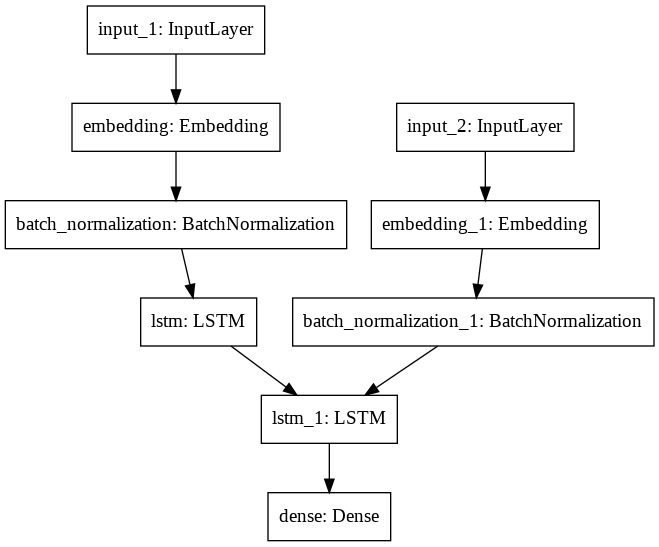
\includegraphics[scale=0.5]{model.png}
\caption{Modèle du RNN}
\end{figure}
L'entraînement peut être réalisé avec la fonction \texttt{train(use\_spatial\_dropout, use\_reccurent\_dropout, use\_batch\_normalisation)} avec l'optimiseur \texttt{ADAM} et la fonction de coût \texttt{sparse\_categorical\_crossentropy}.
\subsubsection{Disposition inférentielle}
Le modèle inférentiel est légèrement complexe. Il est composé de deux modèles : le modèle inférentiel de l'encodeur \texttt{encoder\_model} et le modèle inférentiel du décodeur \texttt{decoder\_model}.
\begin{itemize}
\item le modèle de l'encodeur prend en entrée les mêmes types de donnée que l'encodeur évoqué précédemment et retourne les états (\texttt{h} et \texttt{c}) du LSTM ;
\item le modèle du décodeur prend en entrée les mêmes type de donnée que le décodeur évoqué précédemment ainsi que deux états pour le LSTM. 
\end{itemize}
En injectant les sorties de l'encodeur dans le décodeur on obtient les réponses. Ces deux modèles sont réalisés par la fonction \texttt{make\_inference\_models(encoder\_inputs, encoder\_states, decoder\_embedding, decoder\_lstm, decoder\_dense, decoder\_inputs)}. \\
\tab Ainsi la fonction \texttt{ask\_questions(enc\_model, dec\_model)} répond à une question de la manière suivante :
\begin{itemize}
\item les vecteurs d'états \texttt{h} et \texttt{c} sont obtenus à partir de \texttt{enc\_model.predict} avec comme entrée la question tokenizée (par \texttt{str\_to\_tokens(sentence)} comme expliqué précédemment) ;
\item un mot (ainsi que de nouveaux vecteurs d'états) est produit via \texttt{dec\_model.predict} puis identifié avec une chaîne de caractère grâce à \texttt{tokenizer} ;
\item ce procédé est répété (en utilisant les vecteurs d'états résultant à chaque fois) jusqu'à obtenir le token \texttt{<end>}.
\end{itemize}
\subsubsection{Sauvegarde des objets}
Les différents objets clefs de cette implémentation peuvent être exportés (et importés) via les fonctions suivantes :
\begin{itemize}
\item \texttt{save\_inference\_model(path, encoder\_inputs, encoder\_states, decoder\_embedding, decoder\_lstm, decoder\_dense, decoder\_inputs)} qui sauvergarde le modèle inférentiel dans un fichier ;
\item \texttt{save\_tokenizer(path)} qui sauvegarde \texttt{tokenizer} via le module \texttt{pickle} dans un fichier donné ;
\item \texttt{save\_length(path)} qui sauvegarde la longueur maximale des questions et des réponses ;
\item \texttt{load\_inference\_model(enc\_file, dec\_file)} qui retourne un modèle inférentiel à partir d'un fichier;
\item \texttt{load\_tokenizer(tokenizer\_file)} qui retourne un \texttt{tokenizer} à partir d'un fichier ;
\item \texttt{load\_length(length\_file)} qui retourne la longueur maximale des questions et des réponses à partir d'un fichier. 
\end{itemize}

\subsection{Utilisation}
\subsubsection{Dépendances}

Afin d'installer les dépendances Python, il est nécessaire d’exécuter cette commande :
\begin{center}
\texttt{pip install numpy tensorflow pyyaml requests gensim argparse}
\end{center}
\subsubsection{Utilisation}
Le script Python s'utilise via un système d'arguments qui peuvent être obtenus à partir de \texttt{python script.py -h} :
\begin{verbatim}
usage: script.py [-h] [--downloadData [True/False]] [--customData path]
                 [--speak [True/False]] [--saveModel path] [--loadModel path]
                 [--useSpatialDropout [True/False]]
                 [--useReccurentDropout [True/False]]
                 [--useBatchNormalisation [True/False]] [--vectorSize size]
                 word2vec_model

Seq2Seq Neural Network

positional arguments:
  word2vec_model        Path to the word2vec model

optional arguments:
  -h, --help            show this help message and exit
  --downloadData [True/False]
                        Specify whether the dataset should be downloaded
  --customData path     Specify the path to the custom dataset
  --speak [True/False]  Specify whether to speak with the Network
  --saveModel path      Specify the path where to save the model
  --loadModel path      Specify the path to import the model
  --useSpatialDropout [True/False]
                        Specify whether to use 1D spatial dropout after the
                        embedding layers
  --useReccurentDropout [True/False]
                        Specify whether to use a recurrent dropout in the LSTM
  --useBatchNormalisation [True/False]
                        Specify whether to use batch normalisation
  --vectorSize size     Specify the size of the word vectors
\end{verbatim}

\section{Interface graphique - GUI}
\subsection{Objectifs et outils}

L'objectif de l'interface graphique (\textit{Graphical User Interface}) est de recréer l'interface d'un système de communication tel que \textit{Messenger} ou \textit{WhatsApp} par exemple. Ce package (\texttt{org.lara.gui}), dont le code source individuel peut être retrouvé \href{https://github.com/LaraProject/GUI}{\textit{ici}}, est écrit à l'aide de la bibliothèque \texttt{JavaFX} et a été conçu en partie avec le logiciel \textit{Scene Builder}. Il a pour mission d'être simple d'utilisation, et de permettre à l'utilisateur d'échanger avec une personne de son choix, ainsi que de changer d'interlocuteur et de choisir un surnom. La mise en page a été réalisée à l'aide de CSS.

\subsection{Implémentation et classes}
\subsubsection{La classe \texttt{Main}}

La classe \texttt{Main} permet de lancer l'interface graphique. Y sont définis les chemins des vues \texttt{Homepage.fxml} et \texttt{ChatFrame.fxml}. La classe \texttt{Main} est consitutée de la méthode usuelle d'un GUI : \texttt{start(Stage primaryStage)}.

\subsubsection{La classe \texttt{HomepageCtrl}}

La classe \texttt{HomepageCtrl} constitue le contrôleur de la vue \texttt{Homepage.fxml}, c'est-à-dire de la page d'accueil de l'interface graphique. Elle définit la méthode \texttt{chooseUsername(ActionEvent event)}, qui permet à l'utilisateur de définir un éventuel \textit{username}, et qui permet le changement de vue, au profit de \texttt{ChatFrame.fxml}.

\subsubsection{La classe \texttt{ChatFrameCtrl}}

La classe \texttt{ChatFrameCtrl} constitue le contrôleur de la vue \texttt{ChatFrame.fxml}, c'est-à-dire de la fenêtre de chat de l'interface graphique. Elle définit les boutons et autres composants nécessaires, ainsi que les \textit{handlers} associés :

\begin{itemize}
    \item les méthodes \texttt{idLouis(ActionEvent event)}, \texttt{idAnna(ActionEvent event)}, \texttt{idRiad(ActionEvent event)}, et \texttt{idAntoine(ActionEvent event)} permettent de changer d'interlocuteur et d'effacer la conversation précédente, à partir de la méthode \texttt{idLara()} ;
    \item la méthode \texttt{exitLara(ActionEvent event)} permet d'éteindre le serveur et de quitter l'interface graphique ;
    \item il est possible d'envoyer un message en cliquant sur le bouton dédié, ou simplement en appuyant sur la touche \textit{Entrée} du clavier, grâce aux méthodes \texttt{sendMessage(ActionEvent event)} et \texttt{sendKeyPressed(KeyEvent keyEvent)} qui utilisent la méthode \texttt{send()}.
\end{itemize}

\subsubsection{Les vues}

Les vues \texttt{Homepage.fxml} et \texttt{ChatFrame.fxml} permettent de définir la présentation de l'interface graphique.

\subsubsection{La stylesheet \texttt{application.css}}

Ce fichier CSS permet la mise en page des vues, et d'ainsi obtenir un résultat le plus proche possible des interfaces graphiques des systèmes de communication traditionnels. 

\subsection{Compilation, tests et utilisation}

\subsubsection{Compilation}
Pour les utilisateurs d'\textit{Oracle Java 8} ou d'une version plus récente, le JDK JavaFX est déjà compris dans le JRE, et il faudra alors simplement compiler les classes \texttt{Main}, \texttt{HomepageCtrl}, et \texttt{ChatFrameCtrl} à l'aide des instructions : 

\begin{center}
    \texttt{javac org.lara.gui.Main.java} \\
    \texttt{javac org.lara.gui.HomepageCtrl.java}\\
    \texttt{javac org.lara.gui.ChatFrameCtrl.java}
\end{center}

Pour les utilisateurs d'\textit{OpenJDK}, il faudra d'abord installer \textit{OpenJFX} et l'inclure dans le classpath. Un tutoriel détaillé de l'installation est disponilble \href{https://wiki.openjdk.java.net/display/OpenJFX/Building+OpenJFX}{\textit{ici}}. L'instruction 

\begin{center}
    \texttt{sudo apt-get install openjfx}
\end{center}
permet d'installer \textit{OpenJFX} sous Ubuntu par exemple. \\

Pour les utilisateurs d'une version antérieure à \textit{Oracle Java 8}, il faut télécharger le SDK JavaFX \href{https://gluonhq.com/products/javafx/}{\textit{ici}}, et l'ajouter au classpath. \\

Ainsi, les utilisateurs d'\textit{OpenJDK} ou d'une version de Java antérieure à \textit{Java 8} compileront avec les instructions suivantes :
\begin{center}
    \texttt{javac -classpath "PATH\_TO\_JAVAFX\_SDK/rt/lib/jfxrt.jar" org.lara.gui.Main.java} \\
    \texttt{javac -classpath "PATH\_TO\_JAVAFX\_SDK/rt/lib/jfxrt.jar" org.lara.gui.HomepageCtrl.java} \\
    \texttt{javac -classpath "PATH\_TO\_JAVAFX\_SDK/rt/lib/jfxrt.jar" org.lara.gui.ChatFrameCtrl.java}
\end{center}
où il conviendra de remplacer \texttt{PATH\_TO\_JAVAFX\_SDK} par le chemin du SDK JavaFX. 

\subsubsection{Utilisation}

Les utilisateurs de \textit{Oracle Java 8} ou d'une version plus récente lanceront le client Java par
\begin{center}
    \texttt{java org.lara.gui.Main}
\end{center}

Sinon, il conviendra d'utiliser l'instruction suivante :
\begin{center}
    \texttt{java -classpath "PATH\_TO\_JAVAFX\_SDK/rt/lib/jfxrt.jar:." org.lara.gui.Main}
\end{center}

Il est alors demandé à l'utilisateur de saisir un \texttt{username}, puis de choisir un interlocuteur parmi quatre options. Les messages seront saisis dans le champ adapté, et peuvent être envoyés en appuyant sur le bouton \textit{Send} ou sur la touche \textit{Entrée} du clavier.

\subsubsection{Utilisation avec Maven}
Il est aussi possible de compiler le module via Maven
\begin{center}
\texttt{cd laraGUI} \\
\texttt{mvn compile}
\end{center}
et de l'exécuter via
\begin{center}
\texttt{mvn javafx:run}
\end{center}

\end{document}
